\documentclass[11pt, a4paper, german]{article}
\usepackage[utf8x]{inputenc}
\usepackage{ucs} % unicode
\usepackage[T1]{fontenc}
\usepackage{t1enc}
\usepackage{type1cm}
\usepackage[german]{babel}
 
\usepackage{eurosym} 
\usepackage{amsmath, amssymb}
\usepackage{graphicx}
\usepackage{natbib}
\usepackage{rotating}

\numberwithin {equation}{section}

\sloppy

\begin{document}

\begin{center}
{\large Universität Bayreuth: Philosophy \& Economics, SoSe 2009}
\end{center}
\vspace{0.4em}
\begin{center}
{\huge Alte Klausuren und Übungsklausuren zur Vorbereitung auf die GDE-I Klausur}
\end{center}
\vspace{0.0em}

Nachfolgend sind ein par Übungsaufgaben für die GDE-Klausur zusammengestellt. 
Da es sich dabei um Aufgaben aus alten Klausuren bzw. Übungsklausuren handelt,
könnte es sein, dass sie zur Vorlesung aus dem Sommersemester 2009 nicht 
unbedingt immer passen bzw. dass Themen darin vorkommen, die wir (noch) 
nicht besprochen haben, wie z.B. Spieltheorie.

\begin{flushright}
Eckhart Arnold, 9. Juli 2009
\end {flushright}

\tableofcontents

\section{Die Klausuren}

\subsection{Aufgaben zur Klausurvorbereitung}

Hier sind ein par Aufgaben von der Art, wie sie in der Klausur vorkommen werden.

\subsubsection{Entscheidungen unter Unwissenheit}

\begin{enumerate}
  \item Betrachte folgende Entscheidungstabellen:
\begin{center}
\begin{tabular}{c|c|c|c|c|cc|c|c|c|c|}
\multicolumn{1}{c}{} & \multicolumn{4}{c}{Tabelle 1:} &
\multicolumn{2}{c}{} & \multicolumn{4}{c}{Tabelle 2:}
\\
\cline{2-5} \cline{8-11}
$A_1$ & 4 &  8 & 12  & 0 & & $A_1$ & 0 & -1& 2 & 5 \\ 
\cline{2-5} \cline{8-11} 
$A_2$ & 3 &  2 & 3   & 3 & & $A_2$ & -3& 12& 2 & 4 \\ 
\cline{2-5} \cline{8-11}
$A_3$ & 1 &  5 & 14  & 6 & & $A_3$ & 1 & 8 & -2& 6 \\ 
\cline{2-5} \cline{8-11}
$A_4$ & 2 &  3 & 1   & 7 & & $A_4$ & 2 & 5 & 1 & 0 \\ 
\cline{2-5} \cline{8-11}
\end{tabular}
\end{center}
Löse beide Entscheidungstabellen:
\begin{enumerate}
  \item nach der (lexikalischen) Maximin-Regel
  \item nach der (lexikalischen) Minimax-Bedauerns-Regel
  \item nach dem Indifferenzprinzip
  \item nach der Optimismus-Pessimismus-Regel mit einem Optimismus-Index von 3/4
\end{enumerate}

\item Welche der folgenden Nutzenfunktionen beschreiben jeweils denselben
{\em ordinalen} Nutzen und welche denselben {\em kardinalen} Nutzen:
\begin{enumerate}
  \item \begin{tabular}{l|c|c|c|c|c|c|}
\cline{2-7}
Gut:                      & A & B & C & D & E & F \\
\cline{2-7}
 $u_1$:     & 3 & 2 & 5 & 8 & 1 & 4 \\
\cline{2-7}
 $u_2$:     & 6 & 4 & 8 & 16 & 2 & 7 \\
\cline{2-7}
 $u_3$:     & 7 & 4 & 13 & 22 & 1 & 10 \\
\cline{2-7}
\end{tabular}
 
  \item $u_1(x) = 2x \qquad u_2(x) = -x \qquad u_3(x)=x^2 \qquad 
  u_4(x) = 5x^2-3$
\end{enumerate}

\end{enumerate}

\subsubsection{Wahrscheinlichkeitsrechnung}

\begin{enumerate}
  \item Ein Patient, der kürzlich einen Urlaub in Zentralafrika verbracht hat,
  wird mit Verdacht auf Malaria in die Klinik eingeliefert. Es ist bekannt, dass etwa
  bei 0.5\% derartiger Verdachtsfälle tatsächlich eine Malariaerkrankung
  auftritt. Die behandelnde Ärztin führt zunächst einen Antigen-Schnelltest
  durch. Dieser Schnelltest hat eine
  positiv-positiv Rate von 80\% und eine positiv-negativ Rate von 0.01\%.
  Der Test fällt {\em negativ} aus.
  
  Da der Schnelltest nicht besonders sensitiv ist (wie man an der niedrigen
  positiv-positiv Rate sieht), führt die Ärztin noch einen zweiten Test auf
  Basis einer Polymerase-Kettenreaktion durch. Dieser Test, der mit einer 
  positiv-positiv Rate von 99,5\% und einer positiv-negativ Rate
  von 0.3\% sehr viel zuverlässiger ist, fällt positiv aus.
  
  Mit welcher Wahrscheinlichkeit muss die Ärztin davon ausgehen, dass der
  Patient an Malaria erkrankt ist?

  \item Die Laplace'sche Wahrscheinlichkeit wird wie folgt definiert:
  \begin{enumerate}
    \item Es gibt eine endliche Menge von Elementarereignissen: $\Omega$.
    (Beispiel: Beim Würfeln $\Omega = \{1,2,3,4,5,6\}$)
    \item Jedes Ereignis ist durch eine Menge $E$ charakterisiert, die
    Teilmenge von $\Omega$ ist: $E \subseteq \Omega$. (Beispiel: Das Ereignis,
    eine gerade Zahl zu würfeln, wird durch die Menge
    $E=\{2,4,6\}$ beschrieben.)
    \item Die Wahrscheinlichkeit eines Ereignisses ist definiert als die Anzahl
    der Elemente der Ereignismenge ("`günstige Fälle"') geteilt
    durch die Anzahl der Elementarereignisse ("`mögliche Fälle"'). Wenn $|M|$
    die Anzahl der Elemente der Menge $M$ beschreibt, dann ist die
    Wahrscheinlichkeit $p$ also definiert durch: $p(E) := \frac{|E|}{|\Omega|}$.
  \end{enumerate}
  {\em Beweise}, dass die Laplac'sche Wahrscheinlichkeit die kolmogorowschen
  Axiome erfüllt:
  \begin{enumerate}
    \item Axiom: $\forall_{E \subset \Omega} \qquad p(E) \in \mathbb{R} \qquad
    \mbox{und} \qquad p(E) \geq 0$
    \item Axiom: $p(\Omega) = 1$
    \item Axiom: $\forall_{E,F \subset \Omega} \qquad E \cap F \neq
    \emptyset \Rightarrow p(E \cup F) = p(E) + p(F)$
  \end{enumerate}   
  
  \item Zeige, dass aus den drei kolmogorwschen Axiomen, die {\em Monotonie}
  von Wahrscheinlichkeiten folgt: 
  \[\forall_{E,F \subset \Omega} \qquad E \subset F \Rightarrow p(E)
 \leq p(F) \]
\end{enumerate}

\subsubsection{Entscheidungen unter Risiko}

\begin{enumerate}
  \item In Amerika ist eine Grippewelle ausgebrochen. Experten rechnen damit,
  dass die Grippewelle mit einer Wahrscheinlichkeit von 60\% auch Deutschland
  erreicht. Wenn sie Deutschland erreicht, dann erkrankt ein Anteil von 15\%
  der Bevölkerung. Wird die Grippe nicht behandelt, so sterben 3\% der
  Erkrankten.
 
  Die Gesundheitsministerin erwägt nun, ein breit angelegtes Impfprogramm für
  die gesamte Bevölkerung durchführen zu lassen. Wird die Impfung frühzeitig
  verabreicht, so senkt sie das Erkrankungsrisiko auf 2\%. Allerdings ist die
  Impfung nicht ganz ohne Risiko, denn es kommt -- geheim gehaltenen Zahlen
  zufolge -- bei 0.2\% der geimpften Personen zu schweren Komplikationen, die
  zum Tod führen.
  
  Wenn die Grippe bereits ausgebrochen ist, kann die Gesundheitsministerin
  immer noch die Entscheidung treffen, eine Impfung durchführen zu lassen,
  falls das nicht schon vorher geschehen ist. Allerdings ist die Impfung zu
  diesem späteren Zeitpunkt nicht mehr so effektiv. Sie senkt das
  Erkrankungsrisiko dann nur noch auf 10\% bei gleichem Risiko von
  Komplikationen.

  Aufgaben:
  \begin{enumerate}
  \item Stelle das Entscheidungsproblem als Entscheidungsbaum dar.
  \item Sollte die Gesundheitsministerin eine frühzeitige Durchführung des
  Impfprogramms anstreben?
  \item Angenommen es hätte im Vorfeld eine öffentliche Diskussion über die
  Risiken des Impfprogramms gegeben, so dass die Durchführung des Impfprogramms
  zu einem frühen Zeitpunkt, als noch nicht klar war, ob sie Deutschland
  überhaupt erreicht, politisch nicht durchsetzbar war. Angenommen weiterhin,
  die Grippewelle hat Deutschland schließlich dennoch erreicht und der Ruf nach
  einer schleunigen Massenimpfung wird laut. Sollte die Gesundheitsministerin jetzt 
  doch noch das Impfprogramm durchführen?
  \end{enumerate}
  
  \item Für eine auf einer Menge von Lotterien definierte Präferenzrelation
  gilt neben den üblichen Ordnungsgesetzen von Präferenzrelationen u.a.:
  \begin{enumerate}
    \item {\em Bedingung der höheren Gewinne}: Für beliebige Lotterien $x$,$y$
  und $L^*$ und jede beliebige Wahrscheinlichkeit $a$ gilt: 
  \begin{enumerate}
     \item $L^* \succ x$ genau dann wenn $L(a, L^*, y) \succ L(a, x, y)$.
     \item $L^* \succ y$ genau dann wenn $L(a, x, L^*) \succ L(a, x, y)$.
  \end{enumerate}
  \item {\em Reduzierbarkeit zusammengesetzter Lotterien}:
  Für jede zusammengesetzte Lotterie der Form
  $L(a, L(b,x,y), L(c,x,y))$ gilt $L(a, L(b,x,y), L(c,x,y)) \sim L(d,x,y)$ mit $d:=ab+(1-a)c$. 
  \end{enumerate}
  {\em Zeige} allein mit Hilfe dieser beiden Bedingungen (und der
  Ordnungsgesetze für Präferenzrelationen):
  \begin{enumerate}
    \item Es kann {\em nicht} gelten: $L(a,x,x) \succ x$
    \item Es kann {\em nicht} gelten: $x \succ L(a,x,x)$ 
  \end{enumerate}  

  \item Nimm weiterhin folgende Bedingungen als gegeben an (ergibt sich aus
  der vorhergehenden Aufgabe): Für alle Wahrscheinlichkeiten $a$ und alle
  Lotterien $x$ gilt: $L(a,x,x) \sim x$

  {\em Zeige} allein mit dieser und den Bedingungen aus der vorhergehenden
  Aufgabe: Wenn $B$ ein bestes Grundgut ist, dann kann es keine Lotterie $L(a, x, y)$ geben
  für die gilt: $L(a, x, y) \succ B$
\end{enumerate}



\subsubsection{Spieltheorie}

\begin{enumerate}
  \item Löse das folgende Spiel durch sukkzessive Dominanz (Gib dazu in der
  richtigen Reihenfolge die zu streichenden Zeilen- bzw. Spaltenstrategien an):
\begin{center}
\begin{tabular}{c|c|c|c|c|}
\multicolumn{1}{c}{} & 
\multicolumn{1}{c}{$S_1$} &
\multicolumn{1}{c}{$S_2$} &
\multicolumn{1}{c}{$S_3$} &
\multicolumn{1}{c}{$S_4$} \\ \cline{2-5}
$Z_1$ & 4 & 2 & 0 & 14 \\ \cline{2-5}
$Z_2$ & 11& 7 & 1 & 12 \\ \cline{2-5}
$Z_3$ & 9 & 6 & 4 & 5  \\ \cline{2-5}
$Z_4$ & 3 & 4 & 2 & 8  \\ \cline{2-5}
\end{tabular}
\end{center}

  \item Gegeben seien diese beiden Spiele:

\begin{center}
\begin{tabular}{c|c|c|cc|c|c|}
\multicolumn{1}{c}{} & \multicolumn{2}{c}{{\bf Spiel A}} & 
\multicolumn{2}{c}{} & \multicolumn{2}{c}{{\bf Spiel B}}
\\ 
\multicolumn{1}{c}{} & \multicolumn{1}{c}{$S_1$} & \multicolumn{1}{c}{$S_2$} 
& &
\multicolumn{1}{c}{} & \multicolumn{1}{c}{$S_1$} & \multicolumn{1}{c}{$S_2$} 
\\ \cline{2-3} \cline{6-7}
$Z_1$ &  2, 1  & 0,0 &  &  $Z_1$ & 0,0  & -1,1  \\ \cline{2-3} \cline{6-7}
$Z_2$ & -1,-2  & 1,3 &  &  $Z_2$ & 1,-1 & -2,-2 \\  \cline{2-3} \cline{6-7}
\end{tabular}
\end{center}

  Aufgaben:
  \begin{enumerate}
    \item Bestimmte zu jedem Spiel:
      \begin{enumerate}
        \item die {\em reinen} Nash-Gleichgewichte (sofern vorhanden).
        \item die {\em gemischten} Nash-Gleichgewichte (sofern vorhanden).
      \end{enumerate} 
    \item Bestimme den Erwatungswert der Spiele für jeden Spieler in den
    gemischten Gleichgewichten.
  \end{enumerate} 

\end{enumerate}


\newpage

\subsection{Die Klausur}

\subsubsection*{Aufgabe: Entscheidungen unter Unwissenheit}

%\begin{enumerate}

%\item 
% Geben Sie an, welche der drei Handlungen $A_1$, $A_2$ oder $A_3$
% nach der {\em Maximin-Regel} gewählt werden sollte:
% \begin{center}
% \begin{tabular}{c|c|c|c|}
% \multicolumn{1}{c}{} & \multicolumn{1}{c}{$S_1$}
% & \multicolumn{1}{c}{$S_2$} & \multicolumn{1}{c}{$S_3$} 
% \\ \cline{2-4}
% $A_1$ & 1 & -1 &  5 \\ \cline{2-4} 
% $A_2$ & 3 &  7 & -2 \\ \cline{2-4}
% $A_3$ & 4 & -1 &  1 \\ \cline{2-4}
% \end{tabular}
% \end{center}

%\item 
Lösen Sie nach der Minimax-Bedauerns-Regel. Stellen Sie dazu die
Bedauernstabelle auf und geben Sie dann an, welche drei Handlungen $A_1$, $A_2$
oder $A_3$ gewählt werden sollte.
\begin{center}
\begin{tabular}{c|c|c|c|c|}
\multicolumn{1}{c}{} & \multicolumn{1}{c}{$S_1$}
& \multicolumn{1}{c}{$S_2$} & \multicolumn{1}{c}{$S_3$}
& \multicolumn{1}{c}{$S_4$}
\\ \cline{2-5}
$A_1$ &   3 &   7  &  500 &  4 \\ \cline{2-5} 
$A_2$ & 200 &  100 &    3 & 50 \\ \cline{2-5}
$A_3$ & 150 &   60 &    2 & 25 \\ \cline{2-5}
\end{tabular}
\end{center}

%\end{enumerate}

\subsubsection*{Aufgabe: Entscheidungsbäume}
\label{BaumAufgabe}
Eine Person steht vor einem Entscheidungsproblem, das durch den Entscheidungsbaum {\em auf der letzten Seite} dargestellt wird:
%\begin{center}
%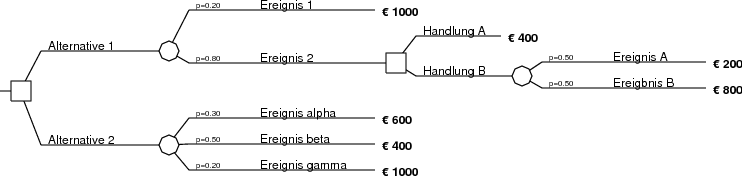
\includegraphics[width=12.5cm]{Grafiken/Klausur.ps}
%\end{center} 
\begin{enumerate}
  \item Sollte die Person an dem weiter rechts liegenden der beiden
  Entscheidungsknoten besser "`Handlung A"' oder "`Handlung B"' wählen?
  \item Wie groß ist der Erwartungswert von "`Alternative 1"' (am ersten
  Entscheidungsknoten von links)?
  \item Sollte die Person "`Alternative 1"' oder "`Alternative 2"' wählen?
\end{enumerate}
(Nehmen Sie dabei an, dass die Person sich rational verhält und den Wert von
zufälligen Ereignissen immer nach dem Erwartungsnutzenprinzip berechnet.)

\subsubsection*{Aufgabe: Nash-Gleichgewichte}

Gegeben sei folgendes Zwei-Personen Spiel:

\begin{center}
\begin{tabular}{c|c|c|}
\multicolumn{1}{c}{} & \multicolumn{1}{c}{$S_1$} &
                               \multicolumn{1}{c}{$S_2$} \\ \cline{2-3} 
$Z_1$                & 1, 1           & 2, 0  \\ \cline{2-3} 
$Z_2$                & 0, 2           & 4, 4  \\ \cline{2-3}
\end{tabular}
\end{center}

\begin{enumerate}
  \item Geben Sie alle {\em reinen} Nash-Gleichgewichte des Spiels an.
  \item Berechnen Sie das {\em gemischte} Nash-Gleichgewicht. Geben Sie an, mit
  welcher Wahrscheinlichkeit der Zeilenspieler im gemischten Gleichgewicht $Z_1$ spielt, und mit welcher 
  Wahrscheinlichkeit der Spaltenspieler im gemischten Gleichgewicht $S_1$ spielt.
\end{enumerate}


\subsubsection*{Aufgabe: Bayes'scher Lehrsatz}

Ein Bergbau-Unternehmen möchte in Sibieren Gold abbauen. Experten schätzen,
dass in dem dafür vorgesehenen Gebiet mit einer Wahrscheinlichkeit von {\bf
30\%} reiche Goldvorkommen zu finden sind. Bevor das Unternehmen jedoch eine
Abbau-Konzession von der Regierung erwirbt, hat es sich das Recht vorbehalten,
Probegrabungen durchzuführen. Falls tatsächlich Goldvorkommen vorhanden
sind, dann liefern die Probegrabungen mit {\bf 95\%} Wahrscheinlichkeit 
ein positives Ergebnis. Allerdings liefern sie mit {\bf 10\%}
Wahrscheinlichkeit auch dann ein positives Ergebnis, wenn in Wirklichkeit kein
Gold vorhanden ist.

\vspace{0.2em}

\setlength{\parindent}{0em}
{\bf Aufgabe:} Mit welcher Wahrscheinlichkeit kann noch davon ausgegangen
werden, dass Gold vorhanden ist, wenn die Probegrabungen ein {\em negatives}
Ergebnis liefern? Stellen Sie zur Lösung der Aufgabe die
entsprechende Rechnung mit Hilfe des Bayes'schen Lehrsatzes auf, und 
rechnen Sie dann die Lösung aus.

\subsubsection*{Aufgabe: Beweise}

\begin{enumerate}
  \item Es seien $x$ und $y$ zwei Güter oder Lotterien mit $x \not\sim y$. Für
  welche Wahrscheinlichkeit $b$ gilt dann: $L(a, x, y) \equiv L(b, y, x)$? Mit
  anderen Worten: Für welchen Wert von $b$ sind die beiden Lotterien über dieselben
  Güter, aber in umgekehrter Reihenfolge identisch?

  \item Die {\em Bedingung der höheren Gewinne} besagt, dass für beliebige
  Lotterien $x$,$y$ und $z$ und jede beliebige Wahrscheinlichkeit $a$ 
  gilt: $x \succ y$ genau dann wenn $L(a, x, z) \succ L(a, y, z)$. 
  (Anders gesagt: Eine Lotterie wir dann vorgezogen, wenn man mit der gleichen 
  Wahrscheinlichkeit auf der {\em ersten} Stelle einen höheren Gewinn erzielen 
  kann, sofern der Gewinn auf der zweiten Stelle derselbe ist.)
  
  {\bf Aufgabe}: Beweisen Sie, dass die Bedingung der höheren Gewinne auch auf der zweiten 
  Stelle gilt, d.h. dass für beliebige Lotterien $x$,$y$
  und $z$ und jede beliebige Wahrscheinlichkeit $a$ gilt: $x \succ y$ genau
  dann wenn $L(a, z, x) \succ L(a, z, y)$.
  
  (Die Gültigkeit der Bedingung der höheren Gewinne auf der ersten Stelle 
   und Ihr Ergebnis der ersten Aufgabe dürfen Sie dabei voraussetzen, aber {\em nicht} den Erwartungsnutzen!)     
\end{enumerate}


\begin{sidewaysfigure}
\begin{center}
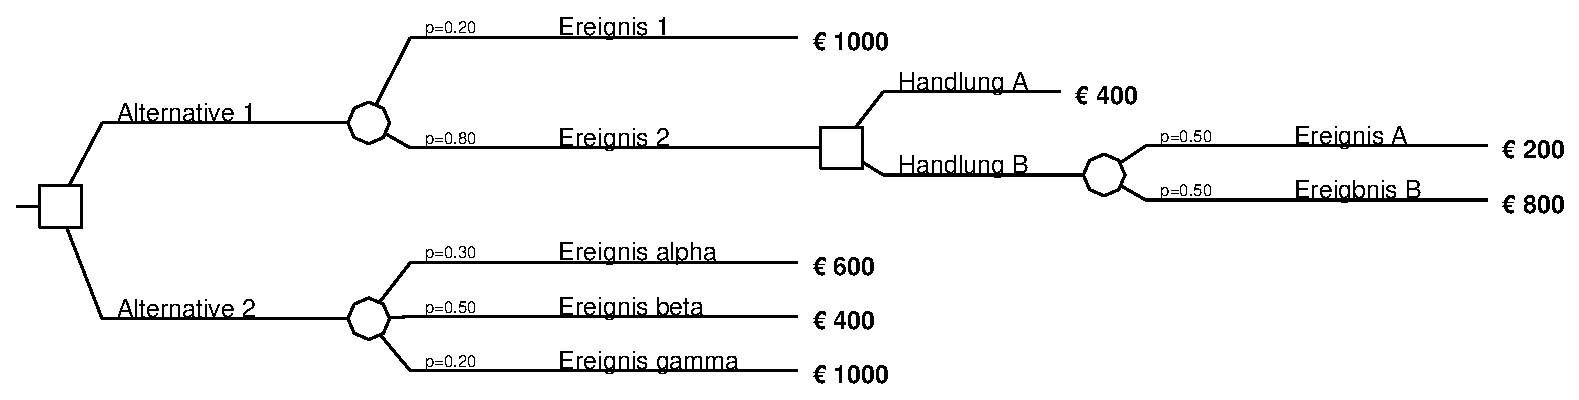
\includegraphics[width=22cm]{Grafiken/Klausur.eps}
\caption{Der Entscheidungsbaum zu Aufgabe \ref{BaumAufgabe}.}
\end{center}
\end{sidewaysfigure}

\newpage


\subsection{Die Nachklausur}

\subsubsection{Aufgabe: Entscheidungsbäume}

Ein Automobilunternehmen möchte ein neu zu entwickelndes Elektroauto auf den
Markt bringen, das zwar weniger schnell fährt aber dafür unglaublich sparsam
ist. Es besteht kein Zweifel daran, dass die Entwicklung eines solchen Wagens
technisch möglich ist. Allerdings würden bis zur Marktreife immer noch
Forschungs- und Entwicklungskosten von 10 Mio Euro anfallen. Wird der neue
Wagen vom Markt akzeptiert, so rechnet die Firma mit einem Ertrag von 15
Mio Euro (worin die Forschungs- und Entwicklungskosten {\em nicht} eingerechnet sind).

Aus Konsumentenbefragungen schließt das Management der Firma, dass die Chance
auf einen Markterfolg bei 60\% liegt. Nun erwägt die Firma, die Markteinführung
des neuen Wagens durch eine breit angelegte Werbekampagne abzustützen. Die
Werbekampagne würde noch einmal mit 1 Mio Euro zu Buche schlagen, aber die
Chance auf einen Markterfolg auf 80\% erhöhen.

\vspace{0.5cm}

{\bf Aufgaben}
\begin{enumerate}
  \item Stellen Sie den Entscheidungsbaum auf.
  \item Wie hoch ist der erwartete Ertrag, wenn die Firma eine Werbekampagne
  durchführt? 
  \item Sollte die Firma demnach eine Werbekampagne durchführen?
\end{enumerate}

\vspace{1cm}

\subsubsection{Aufgabe: Bayes'scher Lehrsatz}

Frau Schmitz ist Einkäuferin für die Gemüseabteilung eines großen
Supermarktes. Ihr ist bekannt, dass ca. 3\% des von Zwischenhändlern
angebotenen Gemüses übermäßig stark durch Pestizide belastet ist. Daher führt
sie vor der Abnahme der Ware immer einen standardisierten Schnelltest
auf Pestizidbelastung durch. Dieser Schnelltest hat eine positiv-positiv Rate
von 90\% und eine positiv-negativ Rate von 5\%. 

\vspace{0.5cm}

{\bf Aufgaben}:
\begin{enumerate}
  \item Aufgabe Ein Zwischenhändler bietet Ihr eine Ladung Gurken an, die von
  ihr {\em positiv} gestestet wird. Mit welcher Wahrscheinlichkeit ist damit zu
  rechnen, dass die Gurken tatsächlich pestizid-belastet sind?
  \item Der Zwischenhändler protestiert und verlangt einen zweiten Test nach
  einem aufwändigeren aber genaueren Verfahren. Die Kenndaten dieses Verfahrens 
  sind eine positiv-positiv Rate von 98 \% und eine positiv-negativ Rate von
  1\%. Angenommen der zweite Test nach dem aufwändigeren Verfahren fällt
  negativ aus: Mit welcher Wahrscheinlichkeit ist dann dennoch mit einer
  Pestizidbelastung zu Rechnen?
\end{enumerate}

\vspace{1cm}


\subsubsection{Aufgabe: Einfache Spiele}

Gegeben sei folgende Spielmatrix ("`Chicken Game"'):

\begin{center}
\begin{tabular}{c|c|c|}
\multicolumn{1}{c}{} & \multicolumn{1}{c}{K} &
                               \multicolumn{1}{c}{D} \\ \cline{2-3} 
K               & 0, 0           & -1,1      
\\ \cline{2-3} 
D               & 1,-1           & -10,-10
\\ \cline{2-3}
\end{tabular}
\end{center}  


\vspace{0.5cm}

{\bf Aufgabe}: Bestimme alle Gleichgewichte des Spiels.

\vspace{0.75cm}

\subsubsection{Aufgabe: Wiederholte Spiele}

Im einem paarweisen, unbestimmt oft {\em wiederholten Gefangendilemma} mit
folgender Auszahlungsmatrix

\begin{center}
\begin{tabular}{c|c|c|}
\multicolumn{1}{c}{} & \multicolumn{1}{c}{Kooperiere} &
                               \multicolumn{1}{c}{Defektiere} \\ \cline{2-3} 
Kooperiere      & 3, 3           & 0, 5     
\\ \cline{2-3} 
Defektiere      & 5, 0           & 1, 1
\\ \cline{2-3}
\end{tabular}
\end{center}  

seien folgende vier Strategien vertreten:
\begin{enumerate}
  \item {\em Tit for Tat}: Kooperiert in der ersten Runde und kooperiert in den
  folgenden Runden immer genau dann, wenn die Gegnerstrategie in der vorhergehenden
  Runde auch kooperiert hat.
  \item {\em Random}: Kooperiert oder defektiert vollkommen zufällig.
  \item {\em Dove}: Kooperiert immer.
  \item {\em Hawk}: Defektiert immer.
\end{enumerate} 

\vspace{0.5cm}

{\bf Aufgaben}: Besimme die Durchschnittspunktzahl, die
\begin{enumerate}
  \item {\em Dove} gegen {\em Random} erhält.
  \item {\em Hawk} gegen {\em Random} erhält.
  \item {\em Tit for Tat} gegen {\em Random} erhält.
\end{enumerate}


\vspace{1cm}

\subsubsection{Aufgabe: Beweisaufgabe}

Das sogennante "`Paradox des Liberalismus"' besagt, dass es {\em kein}
Verfahren zum Treffen kollektiver Entscheidungen gibt, welches den weiter
unten angegebenen Bedingungen genügt. Dabei seien mit Kleinbuchstaben
$x,y,z$ die Güter bezeichnet, über deren Anordnung in einer
kollektiven Präferenzrelation entschieden werden muss. Mit
Großbuchstaben $A,B$ seien die Individuen bezeichnet, die dem
Kollektiv angehören. Die Präferenzen eines Individuums $I$ seien mit
$\succ_I, \prec_I, \sim_I $ symbolisiert. Die kollektiven
Präferenzen seien dagegen mit $\succ_K, \prec_K, \sim_K $
bezeichnet. Als Bedingungen gelten:

\begin{enumerate}
  \item {\em minimale Fairness}: Für jedes beteiligte Individuum gilt: Seine
  Präferenzen setzten sich mindestens bei einem Paar von Alternativen durch,
  d.h. \[ \forall_I \exists_{x,y} \quad x \succ_I y \Rightarrow x \succ_K y \]
  \item {\em unbeschränkter Bereich}: Jedes beliebige individuelle
  Präferenzprofil ist zugelassen (solange die Präferenzen wohlgeformt sind).
  \item {\em Pareto-Effizienz}: Wenn {\em alle} Individuen eine bestimmte
  Alternative einer anderen vorziehen, dann sollte die Alternative auch nach der
  kollektiven Präferenzordnung vorgezogen werden, d.h.
  \[ (\forall_I \quad x \succ_I y) \Rightarrow x \succ_K y \]
\end{enumerate}

Angenommen nun, es existiere ein Kollektiv $K$, dem zwei Individuen $A$
und $B$ angehören und es stünden drei Alternativen $x,y,z$ zur Auswahl.

Weiterhin sei gemäß der Bedingung 1 ("`minimale Fairness"') festgelegt, dass
sich bezüglich der Alternative $x$ oder $z$ die Präferenzen des Individuums $A$
durchsetzen und bezüglich der Altenative $y$ oder $z$ die Präferenzen des
Individuums $B$. 


\vspace{0.5cm}

{\bf Aufgabe}: Zeige: Bei "`ungünstig"' verteilten Präferenzen der
Individuen $A$ und $B$ ist es unmöglich unter Erfüllung aller drei
Bedingungen eine der Alternativen $x,y,z$ als die kollektiv am meisten
bevorzugte auszuzeichnen.

\vspace{1cm}

{\em Tipp}: Gehe in folgenden Schritten vor:
\begin{enumerate}
  \item Wähle zuerst möglichst "`ungünstig"' verteilte Präferenzen für $A$ und
  $B$.
 
  {\footnotesize Nur dann kann das Problem überhaupt entstehen. Wenn $A$ und
  $B$ dieselben oder sehr ähnlich Präferenzen hätten, würde die Abbildung ihrer
  individuellen Präferenzen auf eine kollektive Präferenzordnung keinerlei
  Schwierigkeiten aufwerfen.}

  \item Zeige für jedes des Güter $x,y,z$ einzeln, dass es aufgrund einer oder
  mehrerer der drei Bedingungen bei den für $A$ und $B$ festgelegten
  Präferenzen nicht die kollektiv bevorzugte Alternative sein kann.
  
  {\footnotesize Kann man dies für jede der Alternativen zeigen, dann ist damit
  bewiesen, dass die Entscheidung über eine kollektive Präferenzordnung
  unmöglich ist, denn bei einer solche kollektive Präferenzordnung müsste ja
  irgendeine eine Alternative an der Spitze stehen.}
\end{enumerate}



\end{document}